%==============================================================================
% Sjabloon onderzoeksvoorstel bachproef
%==============================================================================
% Gebaseerd op document class `hogent-article'
% zie <https://github.com/HoGentTIN/latex-hogent-article>

% Voor een voorstel in het Engels: voeg de documentclass-optie [english] toe.
% Let op: kan enkel na toestemming van de bachelorproefcoördinator!
\documentclass{hogent-article}

\usepackage{float}
\usepackage{pgfgantt}

% Invoegen bibliografiebestand
\addbibresource{voorstel.bib}

% Informatie over de opleiding, het vak en soort opdracht
\studyprogramme{Professionele bachelor toegepaste informatica}
\course{Bachelorproef}
\assignmenttype{Onderzoeksvoorstel}
% Voor een voorstel in het Engels, haal de volgende 3 regels uit commentaar
% \studyprogramme{Bachelor of applied information technology}
% \course{Bachelor thesis}
% \assignmenttype{Research proposal}

\academicyear{2023-2024} % TODO: pas het academiejaar aan

% TODO: Werktitel
\title{Automatisering van het orderproces van website naar 3D-geprinte producten}

% TODO: Studentnaam en emailadres invullen
\author{Xander Van der Steichel}
\email{xander.vandersteichel@student.hogent.be}

% TODO: Medestudent
% Gaat het om een bachelorproef in samenwerking met een student in een andere
% opleiding? Geef dan de naam en emailadres hier
% \author{Yasmine Alaoui (naam opleiding)}
% \email{yasmine.alaoui@student.hogent.be}

% TODO: Geef de co-promotor op
\supervisor[Co-promotor]{Rudi De Brandt (sculptures-signs, \href{mailto:mail}{MAIL})}

% Binnen welke specialisatierichting uit 3TI situeert dit onderzoek zich?
% Kies uit deze lijst:
%
% - Mobile \& Enterprise development
% - AI \& Data Engineering
% - Functional \& Business Analysis
% - System \& Network Administrator
% - Mainframe Expert
% - Als het onderzoek niet past binnen een van deze domeinen specifieer je deze
%   zelf
%
\specialisation{Mobile \& Enterprise development}
\keywords{Orderverwerking, 3D-printing, Web, Bambulab}

\begin{document}

\begin{abstract}
    Dit bachelorproefvoorstel richt zicht op de automatisering van het orderproces van website naar 3D-geprinte producten. Het onderzoekt hoe een Python script aan de hand van een pipeline met API calls, orders kan verwerken die vanuit een Shopify-webshop automatisch doorgestuurd worden naar de Bambu Lab X1C 3D-printer. Het probleem dat nu vaak voorkomt is dat dit manueel moet gebeuren wat inefficiëntie en foutgevoelig kan zijn. Hierdoor komt de onderzoeksvraag: "Hoe kan een geautomatiseerde Pipeline worden ontwikkeld die orders vanuit een website automatisch omzet naar een opdracht voor een 3D-printer?" Het is vooral gericht om kleine bedrijven hulp te bieden op een goedkopere manier automatisatie aan te bieden. Het doel van het onderzoek is om een werkend pipeline script te schrijven met behulp van Python, de Shopify API en de Bambu Studio API. De methodologie omvat de literatuurstudie, de ontwikkeling van een proof-of-concept (PoC) , de uitvoering van testen en optimalisatie. Als laatste een ontwikkeling van een eindproduct door optimalisaties. Het verwachte resultaat is een werkend eindproduct, en een efficiënte oplossing dat tijd en kosten bespaart. Ook zou het ervoor moeten zorgen dat er minder menselijke fouten kunnen worden gemaakt. Door deze oplossing zouden de kleine bedrijven meer tijd hebben om andere zaken te gaan regelen.
 
  %Hier schrijf je de samenvatting van je voorstel, als een doorlopende tekst van één paragraaf. Let op: dit is geen inleiding, maar een samenvattende tekst van heel je voorstel met inleiding (voorstelling, kaderen thema), probleemstelling en centrale onderzoeksvraag, onderzoeksdoelstelling (wat zie je als het concrete resultaat van je bachelorproef?), voorgestelde methodologie, verwachte resultaten en meerwaarde van dit onderzoek (wat heeft de doelgroep aan het resultaat?).
\end{abstract}




\tableofcontents

% De hoofdtekst van het voorstel zit in een apart bestand, zodat het makkelijk
% kan opgenomen worden in de bijlagen van de bachelorproef zelf.
%---------- Inleiding ---------------------------------------------------------

% TODO: Is dit voorstel gebaseerd op een paper van Research Methods die je
% vorig jaar hebt ingediend? Heb je daarbij eventueel samengewerkt met een
% andere student?
% Zo ja, haal dan de tekst hieronder uit commentaar en pas aan.

%\paragraph{Opmerking}

% Dit voorstel is gebaseerd op het onderzoeksvoorstel dat werd geschreven in het
% kader van het vak Research Methods dat ik (vorig/dit) academiejaar heb
% uitgewerkt (met medesturent VOORNAAM NAAM als mede-auteur).
% 

\section{Inleiding}%
\label{sec:inleiding}

Waarover zal je bachelorproef gaan? Introduceer het thema en zorg dat volgende zaken zeker duidelijk aanwezig zijn:

\begin{itemize}
  \item kaderen thema
  \item de doelgroep
  \item de probleemstelling en (centrale) onderzoeksvraag
  \item de onderzoeksdoelstelling
\end{itemize}

Denk er aan: een typische bachelorproef is \textit{toegepast onderzoek}, wat betekent dat je start vanuit een concrete probleemsituatie in bedrijfscontext, een \textbf{casus}. Het is belangrijk om je onderwerp goed af te bakenen: je gaat voor die \textit{ene specifieke probleemsituatie} op zoek naar een goede oplossing, op basis van de huidige kennis in het vakgebied.

De doelgroep moet ook concreet en duidelijk zijn, dus geen algemene of vaag gedefinieerde groepen zoals \emph{bedrijven}, \emph{developers}, \emph{Vlamingen}, enz. Je richt je in elk geval op it-professionals, een bachelorproef is geen populariserende tekst. Eén specifiek bedrijf (die te maken hebben met een concrete probleemsituatie) is dus beter dan \emph{bedrijven} in het algemeen.

Formuleer duidelijk de onderzoeksvraag! De begeleiders lezen nog steeds te veel voorstellen waarin we geen onderzoeksvraag terugvinden.

Schrijf ook iets over de doelstelling. Wat zie je als het concrete eindresultaat van je onderzoek, naast de uitgeschreven scriptie? Is het een proof-of-concept, een rapport met aanbevelingen, \ldots Met welk eindresultaat kan je je bachelorproef als een succes beschouwen?

%---------- Stand van zaken ---------------------------------------------------

\section{Literatuurstudie}%
\label{sec:literatuurstudie}

Hier beschrijf je de \emph{state-of-the-art} rondom je gekozen onderzoeksdomein, d.w.z.\ een inleidende, doorlopende tekst over het onderzoeksdomein van je bachelorproef. Je steunt daarbij heel sterk op de professionele \emph{vakliteratuur}, en niet zozeer op populariserende teksten voor een breed publiek. Wat is de huidige stand van zaken in dit domein, en wat zijn nog eventuele open vragen (die misschien de aanleiding waren tot je onderzoeksvraag!)?

Je mag de titel van deze sectie ook aanpassen (literatuurstudie, stand van zaken, enz.). Zijn er al gelijkaardige onderzoeken gevoerd? Wat concluderen ze? Wat is het verschil met jouw onderzoek?

Verwijs bij elke introductie van een term of bewering over het domein naar de vakliteratuur, bijvoorbeeld~\autocite{Hykes2013}! Denk zeker goed na welke werken je refereert en waarom.

Draag zorg voor correcte literatuurverwijzingen! Een bronvermelding hoort thuis \emph{binnen} de zin waar je je op die bron baseert, dus niet er buiten! Maak meteen een verwijzing als je gebruik maakt van een bron. Doe dit dus \emph{niet} aan het einde van een lange paragraaf. Baseer nooit teveel aansluitende tekst op eenzelfde bron.

Als je informatie over bronnen verzamelt in JabRef, zorg er dan voor dat alle nodige info aanwezig is om de bron terug te vinden (zoals uitvoerig besproken in de lessen Research Methods).

% Voor literatuurverwijzingen zijn er twee belangrijke commando's:
% \autocite{KEY} => (Auteur, jaartal) Gebruik dit als de naam van de auteur
%   geen onderdeel is van de zin.
% \textcite{KEY} => Auteur (jaartal)  Gebruik dit als de auteursnaam wel een
%   functie heeft in de zin (bv. ``Uit onderzoek door Doll & Hill (1954) bleek
%   ...'')

Je mag deze sectie nog verder onderverdelen in subsecties als dit de structuur van de tekst kan verduidelijken.

%---------- Methodologie ------------------------------------------------------
\section{Methodologie}%
\label{sec:methodologie}

Hier beschrijf je hoe je van plan bent het onderzoek te voeren. Welke onderzoekstechniek ga je toepassen om elk van je onderzoeksvragen te beantwoorden? Gebruik je hiervoor literatuurstudie, interviews met belanghebbenden (bv.~voor requirements-analyse), experimenten, simulaties, vergelijkende studie, risico-analyse, PoC, \ldots?

Valt je onderwerp onder één van de typische soorten bachelorproeven die besproken zijn in de lessen Research Methods (bv.\ vergelijkende studie of risico-analyse)? Zorg er dan ook voor dat we duidelijk de verschillende stappen terug vinden die we verwachten in dit soort onderzoek!

Vermijd onderzoekstechnieken die geen objectieve, meetbare resultaten kunnen opleveren. Enquêtes, bijvoorbeeld, zijn voor een bachelorproef informatica meestal \textbf{niet geschikt}. De antwoorden zijn eerder meningen dan feiten en in de praktijk blijkt het ook bijzonder moeilijk om voldoende respondenten te vinden. Studenten die een enquête willen voeren, hebben meestal ook geen goede definitie van de populatie, waardoor ook niet kan aangetoond worden dat eventuele resultaten representatief zijn.

Uit dit onderdeel moet duidelijk naar voor komen dat je bachelorproef ook technisch voldoen\-de diepgang zal bevatten. Het zou niet kloppen als een bachelorproef informatica ook door bv.\ een student marketing zou kunnen uitgevoerd worden.

Je beschrijft ook al welke tools (hardware, software, diensten, \ldots) je denkt hiervoor te gebruiken of te ontwikkelen.

Probeer ook een tijdschatting te maken. Hoe lang zal je met elke fase van je onderzoek bezig zijn en wat zijn de concrete \emph{deliverables} in elke fase?

%---------- Verwachte resultaten ----------------------------------------------
\section{Verwacht resultaat, conclusie}%
\label{sec:verwachte_resultaten}

Hier beschrijf je welke resultaten je verwacht. Als je metingen en simulaties uitvoert, kan je hier al mock-ups maken van de grafieken samen met de verwachte conclusies. Benoem zeker al je assen en de onderdelen van de grafiek die je gaat gebruiken. Dit zorgt ervoor dat je concreet weet welk soort data je moet verzamelen en hoe je die moet meten.

Wat heeft de doelgroep van je onderzoek aan het resultaat? Op welke manier zorgt jouw bachelorproef voor een meerwaarde?

Hier beschrijf je wat je verwacht uit je onderzoek, met de motivatie waarom. Het is \textbf{niet} erg indien uit je onderzoek andere resultaten en conclusies vloeien dan dat je hier beschrijft: het is dan juist interessant om te onderzoeken waarom jouw hypothesen niet overeenkomen met de resultaten.



\printbibliography[heading=bibintoc]


% First figure: The Flowchart Image
\begin{figure}[H]  % Use [H] to prevent floating
    \centering
    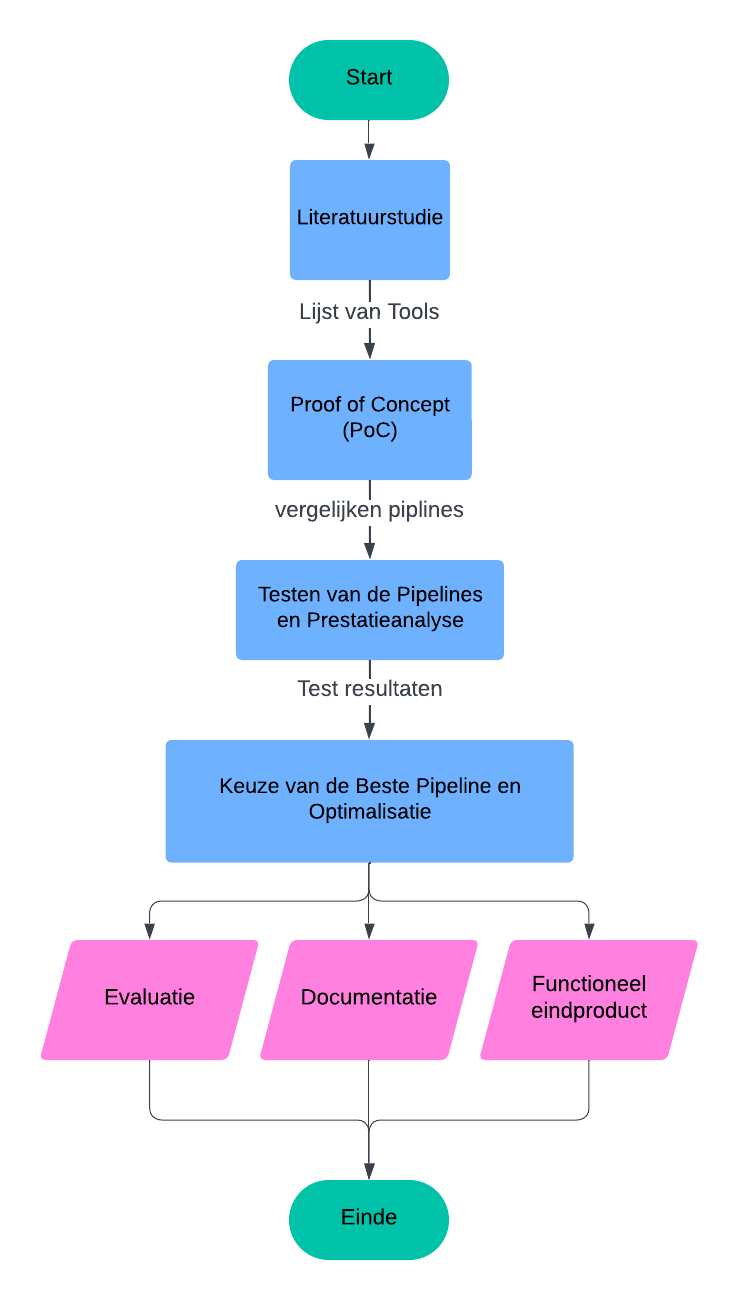
\includegraphics[width=0.5\textwidth]{Flowchart.png}  % Adjust width if necessary
    \caption{Flowchart van verschillende fasen en deliverables van de bachelorproef.}
    \label{fig:flowchart}  % Label for referencing
\end{figure}

\vspace{1em}  % Add some space between figures

% Second figure: The Gantt Chart
\begin{figure}[H]  % Use [H] to prevent floating
    \centering
    \resizebox{\textwidth}{!}{%
        \begin{ganttchart}[
            vgrid,
            hgrid,
            x unit=0.1cm,
            time slot format=isodate,
            compress calendar
            ]{2025-02-01}{2025-05-30}
            
            \gantttitlecalendar{year, month=name} \\
            
            % Fase 1: Literatuurstudie
            \ganttbar[
            progress=70,
            name=litstudie
            ]{Fase 1: Literatuurstudie}{2025-02-01}{2025-02-20} \\
            
            % Fase 2: Proof of Concept (PoC)
            \ganttbar[
            progress=0,
            name=poc
            ]{Fase 2: Proof-of-Concept}{2025-02-21}{2025-03-10} \\
            
            % Fase 3: Experimenten en Testen
            \ganttbar[
            progress=0,
            name=testen
            ]{Fase 3: Experimenten en Testen}{2025-03-11}{2025-05-02} \\
            
            % Fase 4: Iteratieve Ontwikkeling en Optimalisatie
            \ganttbar[
            progress=0,
            name=optimalisatie
            ]{Fase 4: Optimalisatie}{2025-05-03}{2025-05-30} \\
            
        \end{ganttchart}
    }
    \caption{Project Planning Gantt Chart}
    \label{fig:ganttchart}  % Label for referencing
\end{figure}

\end{document}